\documentclass[dvipdfmx]{jsarticle}
\usepackage[T1]{fontenc}
\usepackage[dvipdfmx]{hyperref}
\usepackage{lmodern}
\usepackage{latexsym}
\usepackage{amsfonts}
\usepackage{amssymb}
\usepackage{mathtools}
\usepackage{amsthm}
\usepackage{multirow}
\usepackage{graphicx}
\usepackage{wrapfig}
\usepackage{here}
\usepackage{float}
\usepackage{ascmac}
\usepackage{url}

\title{Javaを用いたデザインパターンコーディングの必要性}
\author{文理学部情報科学科\\5419045 高林 秀}
\date{\today}

\begin{document}

\maketitle

\begin{abstract}
本稿では、今年度発展プログラミングの課題研究として「デザインパターン」に準拠したコーディングスタイルの必要性について、実際に自身でコーディングを行い、論ずる。本演習にはJavaを利用した。
\end{abstract}

\section{目的}
本稿は今年度発展プログラミングの課題研究として、「デザインパターン」に準拠したコーディングスタイルの必要性について論ずることを目的とする。本稿前半では、デザインパターンの利点・効果・必要性などについて説明し、後半では、実際にコーディングを行う。その際、デザインパターンを使用する前のコードとデザインパターンを使用した際のコードを比較・考察していく。
\section{事前知識}
本稿ではJavaを使用する。クラス定義の仕方や、インタフェースなどのJavaで登場する用語についての説明は省略する。これらの解説は以下のURLからレポート「interface、抽象クラスを利用した Java のペア・プログラミング」を参考いただきたい。
\begin{itemize}
  \item url:\url{https://drive.google.com/drive/folders/1QEt-NBptDGq2J1BgOyFnGUx8SMwL5oNc?usp=sharing}
\end{itemize}
\section{デザインパターンとはなにか}
この章では、プログラムコーディングおけるデザインパターンとはどのようなものなのか、歴史的背景や利点・効果、その必要性について述べる。\par
\subsection{歴史的背景}
デザインパターンは、オブジェクト指向型プログラミング言語において、記述したコードを様々なプログラムで再利用できるようにするために考案された「プログラムの設計ルール」のようなものである。1955年に出版された書籍「オブジェクト指向における再利用のためのデザインパターン\cite{book01}」にて、初めて「デザインパターン」と呼ばれる用語が使用された。その書籍の広がりにより、デザインパターンの考え方が広く知られるようになった。\par
その書籍の著者ら(※参考文献の原著4名)は、23種にもおよぶデザインパターンを取り上げており、デザインパターンとはなにか、以下のように述べている。以下、\url{https://ja.wikipedia.org/wiki/%E3%83%87%E3%82%B6%E3%82%A4%E3%83%B3%E3%83%91%E3%82%BF%E3%83%BC%E3%83%B3_(%E3%82%BD%E3%83%95%E3%83%88%E3%82%A6%E3%82%A7%E3%82%A2)}より引用する。
\begin{itemize}
  \item 原文
  \begin{quote}
    [Design patterns] solve specific design problems and make object-oriented designs more flexible, elegant, and ultimately reusable. They help designers reuse successful designs by basing new designs on prior experience. A designer who is familiar with such patterns can apply them immediately to design problems without having to rediscover them.
  \end{quote}
  \item 訳文(Deepl\footnote{ドイツに拠点を置くDeepL GmbHによって開発された、ニューラルネットワークによる翻訳を行うサービス。Google 翻訳よりも精度が高く、微妙なニュアンスのある翻訳ができると話題。}による翻訳)
  \begin{quote}
    特定の設計上の問題を解決し、オブジェクト指向設計をより柔軟に、エレガントに、そして最終的には再利用可能にします。デザインパターンは、新しいデザインを過去の経験に基づいて行うことで、成功したデザインを再利用するのに役立ちます。このようなパターンに精通している設計者は、パターンを再発見することなく、すぐに設計問題に適用することができます。
  \end{quote}
\end{itemize}
この書籍の著者たちは「Gof(Gang of Four)」と呼ばれデザインパターンの名前の1つにもなっている。\par
余談だが、Gofのデザインパターンはかなり前のデザインパターンである。そのため、現代では賛否両論あるようで、一部では批判的な意見も挙げられている。というのも、後に説明するが、デザインパターンはJavaやRubyなどオブジェクト指向型言語で使用される考え方だ。しかしGofのデザインパターンが発表されたのはJavaがリリースされる1995年よりも前、つまりオブジェクト指向プログラミングというものが未熟な時代に発表されたからだ。したがって、現代のプログラミングと合致しない場合もあるという。この意見は\url{https://qiita.com/irxground/items/d1f9cc447bafa8db2388}より参考にさせていただいた。
\subsection{デザインパターンの利点}
前述した通り、デザインパターンの主目的は「コードを様々なプログラムで再利用できるようにする」ことである。ただし、利用するデザインパターンにより、その効果は少し異なる。今回扱う、Gofのデザインパターンは大きく分けて、「生成」、「構造」,「振る舞い」の3つのカテゴリに分類され、その総数は後述するように計23パターンにおよぶ。\par
以上のように分類され、体系が出来上がった概念、考え方なので巷では初心者エンジニアが、オブジェクト指向を学習するときの題材として利用しやすいことも1つの利点と言えるだろう。\par
さて、デザインパターンの大きな利点として、先に上げた「コードの再利用」の他に以下の3つが挙げられるだろう。
\begin{itemize}
  \item 可読性の向上
  \item 保守性の向上
  \item 設計の短時間化
\end{itemize}
\paragraph{可読性の向上}まず、「可読性の向上」だがこれは自分が作成したプログラムを、他のエンジニアやプログラマーが閲覧するときに、そのプログラム、クラスがどんな役割を果たしているのか、どのような意図のコードなのかが把握しやすくなるという意味だ。先に示したように、デザインパターンはすでに確立されたプログラムの設計概念である。したがって、いわば共通言語のようなものであるので、デザインパターンを意識したプログラムは他人からも読みやすいということになる。\par
\paragraph{保守性の向上}次に、「保守性の向上」だがこれは、例えば呼び出し元プログラムの実装方法が変更になった場合でも呼び出し側のプログラムに修正を加えることなく実行できるということだ。大規模な開発になると、実装元と呼び出し側にコードを分散させることが多々あるが、仕様変更やアップデート等で実装側のコードを改変した場合、デザインパターンを意識しないで呼び出し側を設計すると、実装元と呼び出し側両方のプログラムを修正しなければならない。この様なプログラムは、実装側の修正箇所が多くなるたびに呼び出し側も修正しなければならないため非常に効率が悪い。加えて、実装側のコードや動作を把握しなければ呼び出し側の設計ができないという欠点も生じる。\par
デザインパターンを導入すれば、少ない修正でプログラムを動かすことが可能になる。
\paragraph{設計の短時間化}最後に「設計の短時間化」であるが、これはコードの再利用の点と一部重なるかもしれない。デザインパターンは、Gofのデザインパターンの著者を初め、すでに誰かが考え出した設計にしたがってプログラムの設計を行う。したがって、自身で保守性や再利用性を向上させようとあれこれ試行錯誤する必要はなく、コーディング作業全体の効率化を図ることができる。
\subsubsection{デザインパターンの必要性}
ここまで、デザインパターンの利点を述べてきたが、ここではデザインパターンの利用が推奨されるケースについて説明する。\par
現代でプログラミングをする際、すでにこの世に存在している機能をもう一度初めから開発する手間を省くため「ライブラリ」や「フレームワーク」と呼ばれるものが存在する。「ライブラリ」とは、すでに誰かが開発した機能や技術を、他人のプログラム内に組み込めるようにしたものである。有名どころをいくつか列挙すると、Pythonならば、プログラムからウェブブラウザを操作できる機能を提供する「selenium」や、数値計算を高速化、容易にする「numpy」,「pandas」などがあるだろう。Javaならば、webサーバーを構築する際に使用される「Apache HTTP Server」や、HTMLを解析する際に使用される「Jsoup」など多種多様なものが存在する。\par
これらのライブラリやフレームワークが提供する機能を、指定されるコードを用いて、自身の目的に合わせて作成するプログラムに組み込むことができる。\par
つまり、ライブラリやフレームワークを利用するときは、あらかじめ用意されているプログラムを再利用することになる。また、ライブラリやフレームワークが提供する関数やメソッドの処理内容は原則変更することができない。\par
例えば外部に公開されているライブラリを利用し、自身のプログラムを記述する場面を考える。ライブラリから提供される関数やメソッドを呼び出しているのが原因で、自身の意図する目的と異なる動作をすることがある。しかし、ライブラリ側のコードを自身で書き換えると利用している他の関数やメソッドの動作に影響するため、安易に改変することはできない、とする。この様な場合、ライブラリ側のプログラムと、自身で作成したプログラムの動作の差異を吸収するプログラムが必要になってくる。この様な場合は、後に紹介している「Adapterパターン」と呼ばれるデザインパターンを利用することで解決できる場合がある。\par
当然、上で示した各利点を目的とする場合は、それそれのケースに適したデザインパターンを利用することが推奨される。
\subsection{デザインパターンの種類}
先に示したように、デザインパターンは合計23種類ものパターンが存在する。まず「生成」、「構造」,「振る舞い」の3つのカテゴリそれぞれに該当するデザインパターンについて軽く説明を行う。加えて、最後に本稿の演習で使用するデザインパターンであるBridgeパターンについて詳細に取り上げる。
\subsubsection{オブジェクト生成に関するパターン}
オブジェクトの生成を以下のパターンによってコントロールすることができる。状況に応じてオブジェクトの生成をコントロールすることにより、アプリケーション全体の設計に悪影響を与えることを防ぐことができる。以下は、生成に関するパターンに属するデザインパターンである。
\begin{itemize}
  \item Abstract Factory
  \begin{itemize}
    \item インスタンスの生成をコントロールすることを専門に扱うデザインパターンである。プログラム内に整合性が必要とされるとき、関連するクラスのインスタンスをミスなく生成する必要があるときに利用される。Factoryクラスと呼ばれるクラスを切り替えることで、利用するインスタンスを切り替えることができる。
  \end{itemize}
  \item Builder
  \begin{itemize}
    \item 主に、BuriderクラスとDirectorクラスで構成されるデザインパターンである。Builderクラスはいわゆる「表現形式」を定めた抽象クラスで、Directorクラスは「処理課程」を定めた実装クラスである。同様な処理でも、異なる形式の結果を得たい場合に利用する。オブジェクトの生成を容易にしかつ、その生成もコントロールすることを目的としている。
  \end{itemize}
  \item Factory Method
  \begin{itemize}
    \item インスタンスの作成手順を親クラスで定義し、その具体処理を継承先の子クラスで記述するデザインパターンである。生成と、処理内容を分けて記述することにより、より柔軟にオブジェクトの生成を行うことができる。
  \end{itemize}
  \item Prototype
  \begin{itemize}
    \item 日本語では「試作品」「実験版」「原型」という意味を持つ。あらかじめ準備してある「原型」をから、インスタンスを生成するようにするデザインパターンである。例えば、同じ様なオブジェクトが複数欲しいとき、最初に生成したインスタンスをコピーするという方法を行うことで効率よくオブジェクトを得ることができる。つまり、Prototypeパターンは、インスタンスからインスタンスを生成する様なデザインパターンと言える。
  \end{itemize}
  \item Singleton
  \begin{itemize}
    \item 生成されるインスタンスを1つに制限することができるデザインパターンである。このようにすることで、インスタンスの状態を保持することができたり、プログラム内のインスタンスが1つであることを保証できるようにすることができるので、安全性という意味で向上が期待できる。Singletonパターンは、コンストラクタに修飾子privateを付与し、他のクラスからアクセスできないようにすることで、他のクラス内でインスタンスを生成することがないようにしている。
  \end{itemize}
\end{itemize}
\subsubsection{プログラム構造に関するパターン}
オブジェクト同士の関係性を用意にする設計を提供するデザインパターンである。以下のものが構造に関するデザインパターンに該当する。
\begin{itemize}
  \item Adapter
  \begin{itemize}
    \item 本来関係のないクラス同士を関連付けることができるデザインパターンである。先に示したように、提供されているコードと、作成コードの差異を埋めるようなデザインパターンである。
  \end{itemize}
  \item Bridge
  \begin{itemize}
    \item 親クラスに抽象メソッドが定義されている場合、そのメソッドの実装と、実装とは関係ない新機能の記載を分けるようなデザインパターンである。これに関しては、本演習で使用するので、後ほど改めて説明する。
  \end{itemize}
  \item Composite
    \begin{itemize}
      \item 日本語では「複合物」を意味する。全体を囲む「容器」とその「中身」を同じものとして捉え、共通機能を持たせる際に利用する(ファイルシステムなど)。オブジェクトの再帰的な取扱を容易にすることができる。より、具体的にいうと、オブジェクトの集合(グループ)を、オブジェクトの1つのインスタンスとして取り扱うことである。
    \end{itemize}
  \item Decorator
  \begin{itemize}
    \item 同じ様な機能の追加を行うとき、クラスの継承以外の手法で既存のクラスを拡張する際に用いられる。
  \end{itemize}
  \item Facade
  \begin{itemize}
    \item 既存のクラスを複数組み合わせて使うような処理があるとき、複雑さを回避するため、それらのクラスの「窓口や受付」の役割を果たすようなクラスを作成することで構造をシンプルにしようとするデザインパターンである。
  \end{itemize}
  \item Flyweight
  \begin{itemize}
    \item このデザインパターンは計算機のリソース利用の効率化に焦点をあてたデザインパターンである。具体的には、同一のインスタンスを共有したりすることで、無駄なインスタンスの生成を防ぐことができ、プログラムのメモリ使用量などを軽くすることができる。
  \end{itemize}
  \item Proxy
  \begin{itemize}
    \item 日本語では「代理人」を意味する。Proxyパターンは、元のオブジェクトの処理を、別のオブジェクトが肩代わりするようなデザインパターンである。元オブジェクトが行う必要がない処理を代理する別オブジェクトを作成することで、処理の効率化を図ることができる。
  \end{itemize}
\end{itemize}
\subsubsection{オブジェクトの振る舞いに関するパターン}
オブジェクト間の通信を容易に行えるようにするデザインパターンである。例えば、異なるクラスでデータのやり取りを行いたい場合などが該当する。以下のものが振る舞いに関するデザインパターンに該当する。
\begin{itemize}
  \item Chain of Responsibility
  \begin{itemize}
    \item 日本語で、「責任の連鎖」を意味する。つまり、オブジェクト間を鎖で接続し、その鎖をたどって、要求される処理ができるオブジェクトか否かを探す。メリットとして、要求を出すクラスと要求を処理するクラスが分離しているので「クラス間の独立性を確保している」という点が挙げられる。反対にデメリッ卜としては、鎖を渡り歩てオブジェクトを捜索するので、「処理が遅くなる」という点が挙げられる。
  \end{itemize}
  \item Command
  \begin{itemize}
    \item 処理の命令を記載するクラスのインスタンスを1つのオブジェクトとして表現するデザインパターンである。例えば、命令の履歴を管理する際、インスタンスの集合を管理すれば良いことになるので、再度同じ命令を実行するときは、インスタンスを再利用することで実行できる。加えて、1つの引数のみで複数のデータを扱うことができる。
  \end{itemize}
  \item Interpreter
  \begin{itemize}
    \item 任意の形式で書かれたファイルの内容を、いわゆる「通訳」を行うプログラムを介して解析するデザインパターンである。主な使用用途として、interfaceを用いて構文解析の結果を階層構造で示すことができる。
  \end{itemize}
  \item Iterator
  \begin{itemize}
    \item 日本語では、「繰り返し」や「反復」といった意味を持つ。オブジェクトの集合を列挙する方法を提供するデザインパターンである。メリットとしては、オブジェクト間の関係性をシンプルにすることができることが挙げられる。配列など、要素が集合しているオブジェクトにアクセスする場合は特にこのデザインパターンに準拠したコードを記述することが推奨される。
  \end{itemize}
  \item Mediator
  \begin{itemize}
    \item 日本語では、「仲介者」や「まとめ役」といった意味を持つ。オブジェクト同士が互いにアクセスを行わないようにする仕組みを提供するデザインパターンである。これによって、オブジェクト間の関連性の強さをさげることができ、オブジェクトの独立性を保つことができる。
  \end{itemize}
  \item Memento
  \begin{itemize}
    \item 日本語では、「記念品」や「形見」といった意味を持つ。インスタンスの保存と復元を行う場合、インスタンスのもつ情報に無制限にアクセスする必要が生じる。しかしそれではprivateなどの修飾子が使用できない上、カプセル化の意味が無くなってしまう。Mementoパターンは、インスタンスの状態を示す機能を導入することで、カプセル化を無効化することなく、インスタンスの復元と保存を行うことができる。
  \end{itemize}
  \item Observer
  \begin{itemize}
    \item 日本語では、「監督者」といった意味を持つ。「Subject」と呼ばれる監督される側オブジェクトと、「Observer」と呼ばれるSubjectの状態を監督する側のオブジェクトに分けられる。Subjectの状態が変化した際に、Observerに通知される仕組みを持つ。別名Publish-Subscribeパターンと呼ばれることもある。
  \end{itemize}
  \item State
  \begin{itemize}
    \item オブジェクトではなく、状態をクラスとして捉えるデザインパターンである。その時点での状態によってプログラムの振る舞いを変化させるときに適したデザインパターンとなっている。
  \end{itemize}
  \item Strategy
  \begin{itemize}
    \item 日本語では、「戦略」といった意味を持つ。アルゴリズムの実装部分を切り替えることができるデザインパターンである。アルゴリズムの部分を別クラスとして作成し、別のアルゴリズムに切り替えたい場合は、そのクラスを変更してアルゴリズムを切り替えることができる。したがって、メソッド中にアルゴリズムを記載する方法よりも、より柔軟にメンテナンスを行うことができるので、コードの保守性の観点から良いと言えるだろう。
  \end{itemize}
  \item Template Method
  \begin{itemize}
    \item 親クラスで、処理の大枠を決め、具体的な処理内容を継承先の子クラスで決めるデザインパターンである。異なる振る舞いであっても、処理的には似ているとき、それぞれ個別に記載するのではなく、共通化することができる。また、処理の大枠は継承元の親クラスで実装しているので、その部分にバグがあったとしても、継承先の子クラスすべてを修正する必要はない。また、メソッドの機能を部分的に変更することも容易となる。
  \end{itemize}
  \item Visitor
  \begin{itemize}
    \item 日本語では、「訪問者」といった意味を持つ。Visitorパターンは「データ構造とそれを処理する部分を分離する」デザインパターンである。訪問者クラスと呼ばれる、データ構造を淘汰するクラスを作成し、各データの処理はその訪問者クラスが請け負うという構造である。したがって、新たな処理を追加したい場合は、その都度新たな訪問者クラスを作成しさえすれば良い。利用シーンとして、オブジェクトに動的に機能を追加する際に用いられる。
  \end{itemize}
\end{itemize}

\subsection{Bridgeパターン}
本稿後半で行う演習では、デザインパターンとしてBridgeパターンを採用している。ここではBridgeパターンの詳細な説明を行う。\par
Bridgeとは日本語で「橋」を意味する。その意味の通り、Bridgeパターンは目的が異なる2つのクラスを結びつける橋渡しの役割をしている。そのクラスとは、「機能のクラス階層」と「実装のクラス階層」と呼ばれるものである。\par
\paragraph{機能のクラス階層}親クラスで基本的なメソッド(機能)を決定し、継承先の子クラスで新たな機能を追加するクラスの階層のことを「機能のクラス階層」と呼ぶ。
\paragraph{実装のクラス階層}親クラスの抽象メソッドにより、interfaceを決定する。継承先の子クラスにて、メソッドを具体化しそのinterfaceを実装するクラス階層のことを「実装のクラス階層」と呼ぶ。\par

\paragraph{想定場面}
例えば、Bridgeパターンを使用しない場合について考える。親クラス内で、そのオブジェクトの基本機能である抽象メソッドを定義し、継承先の子クラスで抽象メソッドを実装したとする。後から、そのオブジェクトに新たな機能を持たせたいと思い、そのまま子クラスに新たなメソッドを定義したとしよう。最初に行った継承によって作成された子クラスは、オブジェクトの基本機能を定めた「抽象メソッドの実装」が目的である。しかし、次に行った新たなメソッドを定義によって、この子クラスの目的が、「基本機能の実装」と「全く新しい新機能の追加」という複数の目的を持ったクラスになってしまい、一貫性が損なわれてしまう。加えて、抽象メソッドは継承先の子クラスで必ず実装しなければならない性質を持つ。もし、新機能を定義したクラスを作成した場合、基本機能の実装の抽象メソッドを定めている親クラスを継承しているので、そのクラスの数が数個ならばあまり手間はかからないかもしれないが、数十個、数百個となった場合、それぞれ同じ内容の抽象メソッドの実装をしなければならない。このような問題を避けるためにBridgeパターンは利用される。\par

\paragraph{Bridgeパターンまとめ}
まとめると、Bridgeパターンは元からある基本機能を実装するクラスの拡張と、新たな機能を付加するためのクラスの拡張をそれぞれ分離することにより、前述した問題を回避し、クラスの拡張を容易に行えるようにするためのデザインパターンであると言える。
\begin{figure}[H]
  \centering
  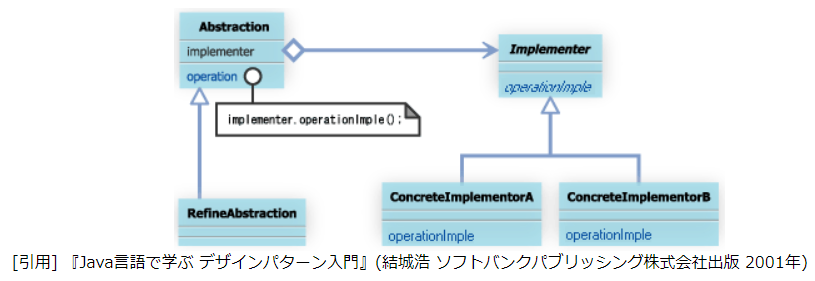
\includegraphics[scale=0.6]{ImgMovies/bridge_ex.PNG}
  \caption{Bridgeパターンのクラス図(UML)}
  ※引用元:\url{https://www.techscore.com/tech/DesignPattern/Bridge.html/}
\end{figure}


\section{実際のコーディングでデザインパターンを利用する}
\subsection{課題説明}
\paragraph{問題} 任意のデザインパターンを1つ選択し、そのパターンを用いる前と用いた後のコード両方を作成して示し、そのパターンを用いたことの効果を説明せよ。
\begin{itemize}
  \item 選択したデザインパターン:Bridgeパターン
\end{itemize}

\subsubsection{演習環境}
今回の演習は仮想マシン上でJavaを使用し行った。下記に演習時の環境を示す。
\begin{itemize}
  \item ホストOS:Window10 Home 20H2
  \item 仮想OS:Ubuntu 20.04.2 LTS
  \item CPU:Intel(R)Core(TM)i7-9700K @ 3.6GHz
  \item GPU:Nvidia Geforce RTX2070 OC @ 8GB
  \item ホストRAM:16GB
  \item 仮想RAM:4GB
  \item 使用言語:Java
  \begin{itemize}
    \item バージョン情報は下記に示す。
    \begin{verbatim}
  openjdk version "11.0.11" 2021-04-20
  OpenJDK Runtime Environment (build 11.0.11+9-Ubuntu-0ubuntu2.20.04)
  OpenJDK 64-Bit Server VM (build 11.0.11+9-Ubuntu-0ubuntu2.20.04, mixed mode, sharing)
    \end{verbatim}
  \end{itemize}
\end{itemize}

\subsection{制作物}
今回の演習の制作物として、「FizzBuzzゲーム」をコンソールで行えるようにしたものを作成する。\par
FizzBuzzゲームとは、1から任意の数までの範囲を対象に、それぞれの数字が3の倍位数なら「Fizz」と出力し、5の倍数なら「Buzz」と出力し、3と5の公倍数の場合は「FizzBuzz」と出力する単純なゲームである。具体的な流れは下記。
\begin{enumerate}
  \item ユーザーが表示する数値の上限を入力する。この入力値を$i$とする。
  \item コンソール上に出力する数値$d$の範囲を$1 \leq d \leq i$とし,$d = i$になるまで繰り返し改行して表示する。
  \item このとき、$d$の値が3の倍数のならば出力は「Fizz」とし、5の倍数ならば出力は「Buzz」、3と5の公倍数ならば出力は「FizzBuzz」とする。
\end{enumerate}
以下は、その実行例である。
\begin{figure}[H]
  \centering
  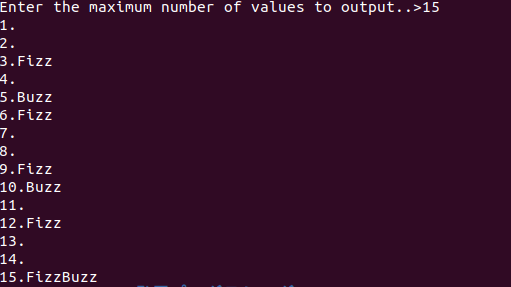
\includegraphics[scale=0.6]{ImgMovies/FizzBuzzEx.png}
  \caption{FizzBuzzの表示例}
\end{figure}
プログラム起動時に、ユーザーが表示する数値の上限を入力し、1〜その数値までの数が「Fizz」または「Buzz」または「FizzBuzz」に該当するのか出力している。\par
まず、基本機能として引数に渡された整数が「Fizz」なのか「Buzz」なのか「FizzBuzz」なのか判定し出力するプログラムを作成する。その後、新機能として新たに「Fizz」または「Buzz」または「FizzBuzz」に該当する数字に出力が来たとき、ユーザーに「Fizz」または「Buzz」または「FizzBuzz」のどれに該当するか当ててもらう機能を実装する。\par
\subsubsection{デザインパターン前のソースコード}
\paragraph{実装}
この時点でのファイル構造は以下の様になっている。
\begin{verbatim}
      ./
      ├── FizzBuzz.java
      ├── Main.java
      ├── PlayFizzBuzz.java
\end{verbatim}
各Javaファイルを格納したフォルダに、呼び出しと表示を行うMain.java、抽象クラスであるFizzBuzzを定義したFizzBuzz.java、FizzBuzzクラスを継承し、親クラスの抽象メソッドの実装を担うPlayFizzBuzz.javaを作成した。FizzBuzzゲームの処理の大枠を親クラスであるFizzBuzzクラスに抽象メソッドとして定義し、具体的な処理内容を小クラスであるPlayFizzBuzzクラスで記述している。\par
各ファイルのソースコードは下記のとおりである。
\begin{itembox}[l]{Main.java}
  \begin{verbatim}
import java.util.*;

public class Main {
    public static void main(String[] args) {
        System.out.print("Enter the maximum number of values to output..>");
        Scanner scan = new Scanner(System.in);
        int upper_range = scan.nextInt();
        PlayFizzBuzz fizzbuzz_obj = new PlayFizzBuzz();

        for(int i = 0; i < upper_range; i++) {
            System.out.print(i+1);
            System.out.print(".");
            fizzbuzz_obj.displayFizzBuzz(i+1);
            System.out.println();
        }
    }

}
  \end{verbatim}
\end{itembox}
\begin{itembox}[l]{FizzBuzz.java}
  \begin{verbatim}
public abstract class FizzBuzz {
    protected abstract String judge_fizzbuzz(int i);
    public abstract void displayFizzBuzz(int i);
}
  \end{verbatim}
\end{itembox}
\begin{itembox}[l]{PlayFizzBuzz.java}
  \begin{verbatim}
public class PlayFizzBuzz extends FizzBuzz {

    protected String judge_fizzbuzz(int i) {
        String result = "";
        if(i >=3 ) {
            if(i % 3 == 0 && i % 5 == 0) {
                result = "FizzBuzz";
            } else if(i % 3 == 0) {
                result = "Fizz";
            }else if(i % 5 == 0) {
                result = "Buzz";
            }
        }
        return result;
    }

    public void displayFizzBuzz(int i) {
        String result = judge_fizzbuzz(i);
        System.out.print(result);
    }
}
  \end{verbatim}
\end{itembox}
実装部分であるPlayFizzBuzzクラスの各メソッドについて説明する。最初のjudge\_fizzbuzzメソッドであるが、これは引数に与えられた整数値1つが、「Fizz」「Buzz」「FizzBuzz」のどれに該当するのか、その結果を文字列で返す。どれにも該当しない場合は、その結果を空文字で返す。このメソッドはPlayFizzBuzzクラス内、でしか使用しないため修飾子protectedを付与した。本来privateでも良いのだが、親クラスであるFizzBuzzクラス内で、この抽象メソッドを定義してしまっているのでprivateが使用できない。続くdisplayFizzBuzzメソッド内で、judge\_fizzbuzzメソッドの結果を標準出力している。\par
実行時の出力は下図。
\begin{figure}[H]
  \centering
  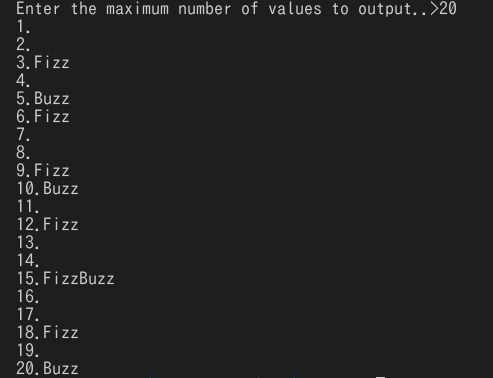
\includegraphics[scale=0.6]{ImgMovies/prod01-result1.png}
  \caption{実行時の様子}
\end{figure}
%%ここにその説明。
実行開始後に、出力する数値の上限の入力を求められる。ユーザーはその指示に従い整数を入力する。Enterを押し数値を渡すと、その数値までの「Fizz」「Buzz」「FizzBuzz」の結果を表示している。画像の実行例では上限値が20で、1~20までの範囲でそれぞれの数字が「Fizz」「Buzz」「FizzBuzz」のどれに該当するのか出力している。
\paragraph{新機能の追加}
では、新機能である、ユーザーに「Fizz」または「Buzz」または「FizzBuzz」のどれに該当するか当ててもらう機能を追加する。特になにも意識せず、PlayFizzBuzzクラス内に、「doQuestionメソッド」、「questionFizzBuzzメソッド」を追加した。
%%ここに変更を加えたソースコードを表示。

\begin{itemize}
  \item PlayFizzBuzz.java
\end{itemize}
\begin{verbatim}
  import java.util.*;
  public class PlayFizzBuzz extends FizzBuzz {

      protected String judge_fizzbuzz(int i) {
          String result = "";
          if(i >=3 ) {
              if(i % 3 == 0 && i % 5 == 0) {
                  result = "FizzBuzz";
              } else if(i % 3 == 0) {
                  result = "Fizz";
              }else if(i % 5 == 0) {
                  result = "Buzz";
              }
          }
          return result;
      }

      public void displayFizzBuzz(int i) {
          if(doQuestion(i)){
              boolean ans = questionFizzBuzz(i);
              if(ans == true) {
                  System.out.print("##You are right.##");
              } else {
                  System.out.print("##You worng!! Bye.##");
                  System.exit(0);
              }
          }
          String result = judge_fizzbuzz(i);
          System.out.print(result);
      }

      private boolean doQuestion(int i) {
          String result = judge_fizzbuzz(i);
          if(result != "") {
              return true;
          } else {
              return false;
          }
      }

      protected boolean questionFizzBuzz(int i) {
          String ans = judge_fizzbuzz(i);
          Scanner scan = new Scanner(System.in);
          String userAns = "";
          if(ans != "") {
              System.out.print(
                  "
                  Is this number 'Fizz'? Or is it 'Buzz',
                   or is it 'FizzBuzz'? >
                   "
                  );
              userAns = scan.nextLine();
          }
          if(ans.equals(userAns) == false) {
              return false;
          } else {
              return true;
          }
      }
  }

\end{verbatim}
doQuestionメソッドで、ユーザーに質問を問いかけるか判定し、questionFizzBuzzメソッド内で、ユーザーの解答が正解かどうか判定している。その結果を基本機能であったdisplayFizzBuzzを拡張して表示するようにした。\par
実行時の様子は下図。
\begin{figure}[H]
  \centering
  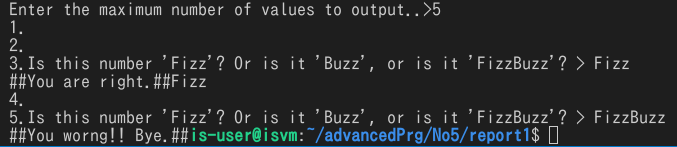
\includegraphics[scale=0.6]{ImgMovies/prod01-result2.png}
  \caption{実行時の様子}
\end{figure}
これまで通り、ユーザーが表示する数値の上限を入力し、コンソールにその上限までの数値が表示される。表示されている数値が、「Fizz」「Buzz」「FizzBuzz」のいずれかに該当する場合、ユーザーに質問を問いかけている。ユーザーが正解の文字列を入力すれば、次の数字へ進み、不正解ならばメッセージを出力してプログラムを終了している。
\subsubsection{デザインパターン後のソースコード}
では、Bridgeパターンを使用してFizzBuzzゲームを作成してみる。
まず、ディレクトリ構造から説明する。
\begin{verbatim}
    ./
    ├── FBPlayImp.java
    ├── FizzBuzz.java
    ├── FizzBuzzImpl.java
    ├── Main.java
    └── UserQuestion.java
\end{verbatim}
なお、UserQuestion.javaにて前述と同様の新機能追加を行っている。\par
それぞれのソースコードは下記のとおりである。
\begin{itemize}
  \item Main.java
  \begin{verbatim}
import java.util.*;

public class Main {
    public static void main(String[] args) {
        System.out.print("Enter the maximum number of values to output..>");
        Scanner scan = new Scanner(System.in);
        int upper_range = scan.nextInt();
        FizzBuzz fizzbuzz_obj = new FizzBuzz(new FBPlayImp());

        for(int i = 0; i < upper_range; i++) {
            System.out.print(i+1);
            System.out.print(".");
            fizzbuzz_obj.displayFizzBuzz(i+1);
            System.out.println();
        }
    }

}
  \end{verbatim}
  \item FizzBuzz.java
\begin{verbatim}

public class FizzBuzz {
    private FizzBuzzImpl fzImpl;
    public FizzBuzz(FizzBuzzImpl fzImpl) {
        this.fzImpl = fzImpl;
    }

    protected String judge_fizzbuzz(int i) {
        String result;
        result = fzImpl.judge_fizzbuzz(i);
        return result;
    }

    public void displayFizzBuzz(int i) {
        fzImpl.displayFizzBuzz(i);
    }
}

  \end{verbatim}
  \item FBPlayImp.java
  \begin{verbatim}

public class FBPlayImp extends FizzBuzzImpl {

    protected String judge_fizzbuzz(int i) {
        String result = "";
        if(i >=3 ) {
            if(i % 3 == 0 && i % 5 == 0) {
                result = "FizzBuzz";
            } else if(i % 3 == 0) {
                result = "Fizz";
            }else if(i % 5 == 0) {
                result = "Buzz";
            }
        }
        return result;
    }

    public void displayFizzBuzz(int i) {
        String result = judge_fizzbuzz(i);
        System.out.print(result);
    }

}
  \end{verbatim}
  \item FizzBuzzImpl.java
  \begin{verbatim}
  public abstract class FizzBuzzImpl {
    protected abstract String judge_fizzbuzz(int i);
    public abstract void displayFizzBuzz(int i);
  }
  \end{verbatim}
  \item UserQuestion.java
  \begin{verbatim}
    import java.util.*;

public class UserQuestion extends FizzBuzz{

    public UserQuestion(FizzBuzzImpl fzImpl) {
        super(fzImpl);
    }

    @Override
    public void displayFizzBuzz(int i) {
        if(doQuestion(i)){
            boolean ans = questionFizzBuzz(i);
            if(ans == true) {
                System.out.print("##You are right.##");
            } else {
                System.out.print("##You worng!! Bye.##");
                System.exit(0);
            }
        }
        String result = judge_fizzbuzz(i);
        System.out.print(result);
    }

    private boolean doQuestion(int i) {
        String result = judge_fizzbuzz(i);
        if(result != "") {
            return true;
        } else {
            return false;
        }
    }

    protected boolean questionFizzBuzz(int i) {
        String ans = judge_fizzbuzz(i);
        Scanner scan = new Scanner(System.in);
        String userAns = "";
        if(ans != "") {
            System.out.print(
                "Is this number 'Fizz'? Or is it 'Buzz', or is it 'FizzBuzz'? > "
                );
            userAns = scan.nextLine();
        }
        if(ans.equals(userAns) == false) {
            return false;
        } else {
            return true;
        }
    }
}
  \end{verbatim}
\end{itemize}
構造としては、まず基本機能の実装を抽象クラスであるFizzBuzzImplクラスで抽象メソッドを定義し、その継承先であるFBPlayImpクラスにて、抽象メソッドの実装を行っている。各メソッドの処理内容は、Bridgeパターンを用いないものと同じである。また実行時の様子は、これもBridgeパターンを用いないものと同じで下図のようになった。\par
\begin{figure}[H]
  \centering
  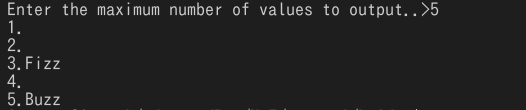
\includegraphics[scale=0.6]{ImgMovies/prod02-result1.png}
  \caption{実行時の様子}
\end{figure}
次に、新機能の追加について説明する。新機能で使用するメソッドは、FizzBuzzクラスを継承したUserQuestionクラスにて行っている。その際、FizzBuzzクラスのdisplayFizzBuzzメソッドの一部を拡張する必要があったため、メソッドのオーバーライドを行っている。この機能を呼び出すときは、Mainクラス内で、UserQuestionクラスのインスタンスを作成し、displayFizzBuzzメソッドを呼び出す。
\begin{itemize}
  \item Main.java
  \begin{verbatim}
import java.util.*;

public class Main {
    public static void main(String[] args) {
        System.out.print("Enter the maximum number of values to output..>");
        Scanner scan = new Scanner(System.in);
        int upper_range = scan.nextInt();
        FizzBuzz fizzbuzz_obj = new UserQuestion(new FBPlayImp());

        for(int i = 0; i < upper_range; i++) {
            System.out.print(i+1);
            System.out.print(".");
            fizzbuzz_obj.displayFizzBuzz(i+1);
            System.out.println();
        }
    }
}
  \end{verbatim}
\end{itemize}
  実行時の様子は下図。
  \begin{figure}[H]
    \centering
    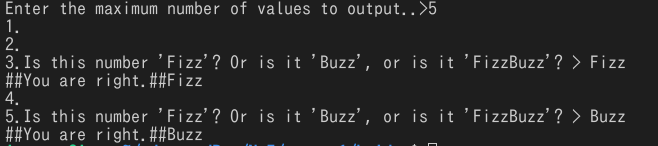
\includegraphics[scale=0.6]{ImgMovies/prod02-result2.png}
    \caption{実行時の様子}
  \end{figure}
\subsection{考察}
まずBridgeパターンを用いない場合のソースコードを見てみると、ある問題点が浮かび上がる。それは基本機能の実装と、新機能の追加を一つのクラス内で行っていることにある。このようにすると、PlayFizzBuzzクラスの継承の意味が「基本機能の実装」と「新機能の追加」という2つの目的に基づいて行われたことになるため、そのクラスが何を行うクラスなのかはっきりしなくなってしまう。しあたがって、コードの可読性の点で良いとは言えない。\par
対して、Bridgeパターンを使用したソースコードを見てみると、「基本機能の実装」はFBPlayImpクラスが行い、「新機能の追加」はUserQuestionクラスが行っている。これらのクラスの継承元はそれぞれ、FizzBuzzImplクラス、FizzBuzzクラスと別のクラスを継承していることが分かる。このようにすることで、1つの継承には1つの目的が割り当てられ、その継承がなにを目的として行われたのかが明確になる。したがって、実装と機能追加が混在することがなく、コードの可読性の向上ができたと考えられる。\par
しかしその反面デメリッ卜もある。それは、コードがBridgeパターンを使用しないものよりも、分散されてしまっている点が挙げられるだろう。継承を多く利用しているので、役割が明確に分けられているとは言え、単純なプログラムなのにコードが複数のファイルに分散されてしまっている。

\section{まとめ}
\section{巻末資料}
本稿で使用したコードは以下のリポジトリに掲載している。
\begin{itemize}
  \item GitHub:\url{https://github.com/tsyu12345/advancedPrg}
\end{itemize}
\begin{thebibliography}{99}
  \bibitem{book01}  Erich Gamma (原著), Ralph Johnson (原著), Richard Helm (原著), John Vlissides (原著), 本位田 真一 (翻訳), 吉田 和樹 (翻訳)「オブジェクト指向における再利用のためのデザインパターン」改訂版(ソフトバンククリエイティブ,1999/10/1)
\end{thebibliography}

\end{document}
